% !TEX root = ../master-thesis.tex

\begin{figure}[h]
    \centering
    \addletter{140}{a}
    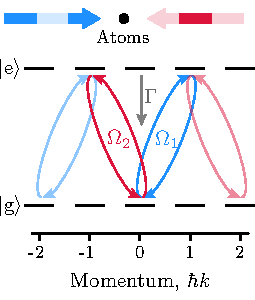
\includegraphics{fig-ai/ssh-scheme.pdf}
    \hfill
    \addletter{140}{b}
    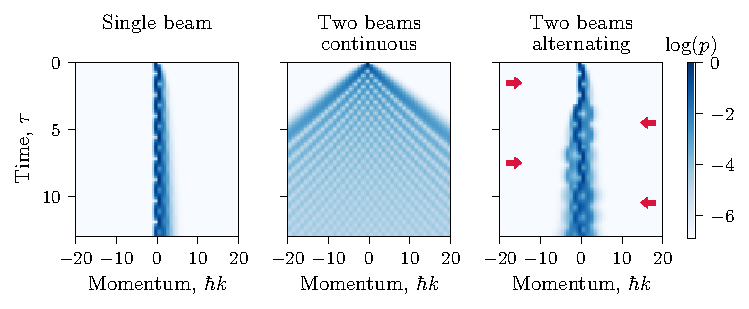
\includegraphics{fig-py/ssh-model.pdf}
    \caption{
        \textbf{Momentum-space dynamics in the SSH model}. 
        a) Atoms undergo momentum-changing transitions via couplings $\Omega_1$ and $\Omega_2$, realizing a SSH-like quantum walk.
        b) Momentum distributions over time for different beam configurations: single beam (left) shows small shift; two continuous beams (middle) result in fast spreading; alternating beams (right) suppress spread.
    }
    \label{fig:sshmodel}
\end{figure}


\begin{figure}[h]
    \centering
    \addletter{125}{a}
    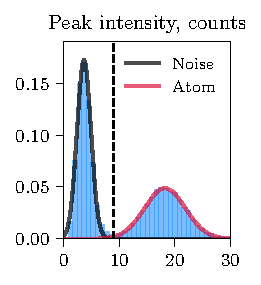
\includegraphics{fig-py/imaging-hist.pdf}
    \hfill
    \addletter{125}{b}
    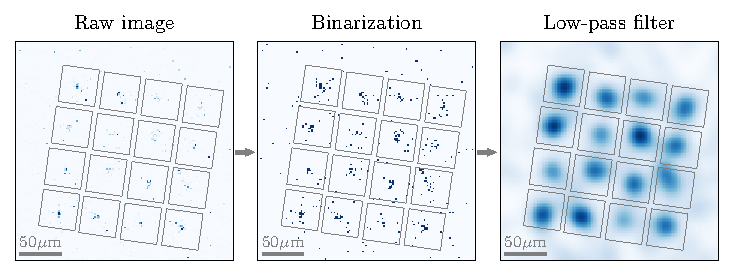
\includegraphics{fig-py/imaging-base.pdf}
    \caption{
        \textbf{Single-atom identification and image processing.}
        a) Histogram of peak intensities extracted from binarized and low-pass filtered images shows a bimodal distribution: the first peak corresponds to camera noise (black), the second corresponds to single atoms (red). The dashed line indicates the threshold used for atom identification.
        b) Image processing pipeline: Raw fluorescence image (left), binarization by intensity thresholding (center), and application of a low-pass filter (right) to reveal spatially localized atomic signals. 
        % \red{Для (a) можно добавить fit, показав что иногда случаются и два атома.}
    }
    \label{fig:imaging}
\end{figure}



\newpage

\begin{figure}[h]
    \centering
    \addletter{200}{a}
    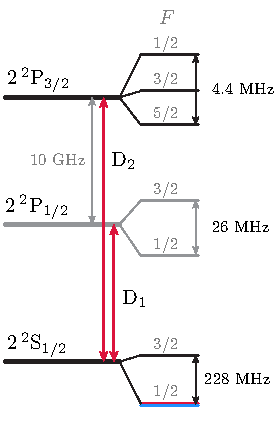
\includegraphics{fig-ai/li-levels-base.pdf}
    \hspace{1cm}
    \addletter{200}{b}
    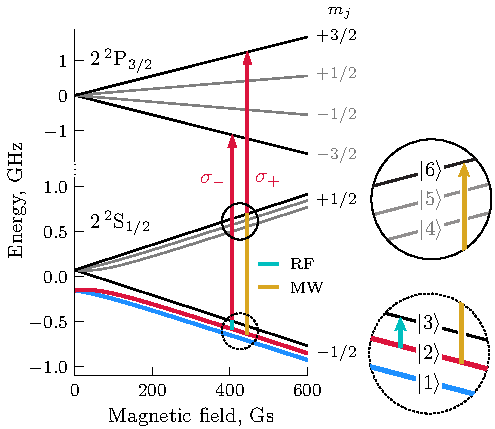
\includegraphics{fig-ai/li6-zeeman-broken-ai.pdf}
    \caption{
        \textbf{${}^6$Li energy levels}. 
        a) Level diagram of the ground and excited states of ${}^6$Li \cite{gehm_preparation_2003}, including the D1 and D2 transitions around $\lambda = 671$~nm. 
        b) Zeeman splitting of the hyperfine levels of the $2\, {}^2\mathrm{S}_{1/2}$ and $2\, {}^2\mathrm{P}_{2/2}$ in ${}^6$Li \cite{serwane_deterministic_2011, sibalic_arc_2017}. As different spin states for physics we consider state $\ket{1}$ and $\ket{2}$, but for imaging it is worth to flip them to stretched states $\ket{6}$, $\ket{3}$. Colored lines indicate transitions driven by radiofrequency (RF) and microwave (MW) fields.
    }
    \label{fig:li6levels}
\end{figure}


\begin{figure}[h]
    \centering
    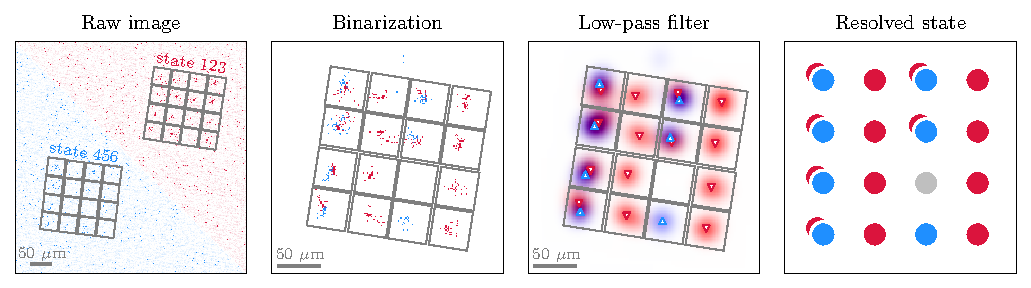
\includegraphics{fig-py/imaging-spin-resolved.pdf}
    \caption{
        \textbf{Spin-resolved single-atom imaging.}
        Spatially separated $\sigma_+$ and $\sigma_-$ fluorescence is imaged onto two distinct regions of the camera. The binarization step identifies photon counts above a threshold, followed by a low-pass filter to extract spatially localized signals. Final spin states are assigned based on relative signal strength in each channel:
        \raisebox{-1pt}{\scalebox{1.5}{\textcolor{ublue}{\textbullet}}} -- $\ket{1}$, 
        \raisebox{-1pt}{\scalebox{1.5}{\textcolor{ured}{\textbullet}}} -- $\ket{2}$, 
        \raisebox{-1pt}{\scalebox{1.5}{\textcolor{uhole}{\textbullet}}} -- no atom.
    }
    \label{fig:spin-resolved}
\end{figure}


\newpage




\begin{figure}[h]
    \centering
    % 
    \addletter{140}{a} 
    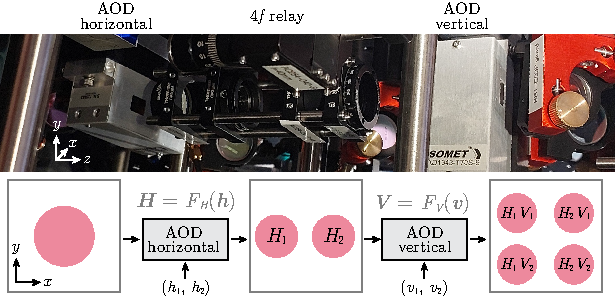
\includegraphics{fig-ai/crossed-aod.pdf}
    \hfill
    \addletter{140}{b} 
    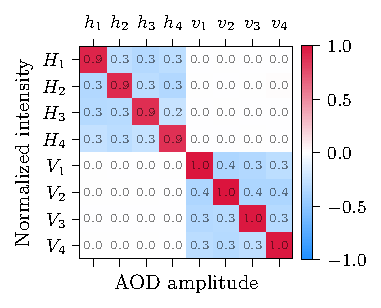
\includegraphics{fig-py/crosstalk-camera.pdf}
    % 
    \newline
    \phantom{42}
    \newline
    % 
    \addletter{115}{c}
    \raisebox{1cm}{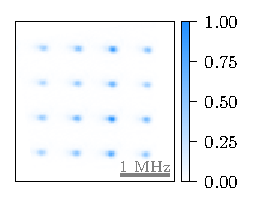
\includegraphics{fig-py/crosstalk-camera-img.pdf}}
    \phantom{42}
    \addletter{115}{d}
    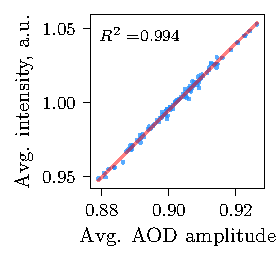
\includegraphics{fig-py/crosstalk-camera-amp.pdf}  
    \phantom{42}
    \addletter{115}{e}
    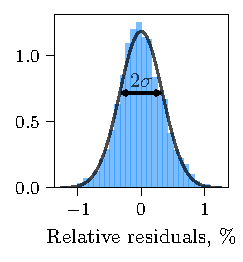
\includegraphics{fig-py/crosstalk-camera-res.pdf}
    % 
    \caption{
        \textbf{Tweezer array control using orthogonal AODs.}
        (a) Experimental setup: two orthogonal AODs generate a 2D tweezer array. The applied harmonic amplitudes $h_i$, $v_j$ define the output intensities $H_i = F_H(h)$ and $V_j = F_V(v)$ in horizontal and vertical directions, respectively. 
        (b) Crosstalk matrix $F'$ reconstructed via linear regression from camera images, showing how modulation of one harmonic affects others. 
        (c) Example of measured intensity distribution at uniform input amplitudes ($h_i = v_j = 0.9$), illustrating imbalance in the resulting pattern. 
        (d) The total intensity $\Lambda = \sum_{ij} H_i V_j$ scales linearly with the mean input amplitude. 
        (e) Residuals of the linear model (fitted in the range $[0.85, 0.95]$) are normally distributed. 
        All data were obtained in this work using direct camera-based measurements.
    }
    \label{fig:control}
\end{figure}

\begin{figure}[h!]
    \centering
    \addletter{140}{a}
    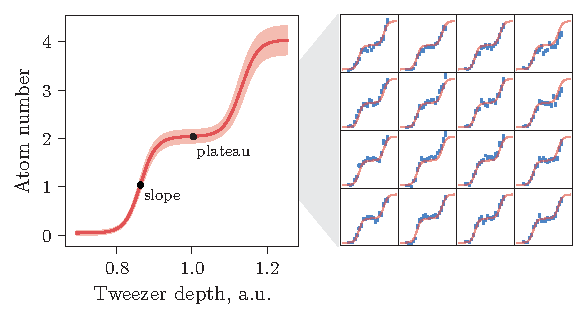
\includegraphics{fig-ai/step-plot-joined.pdf}
    \phantom{42}
    \addletter{140}{b}
    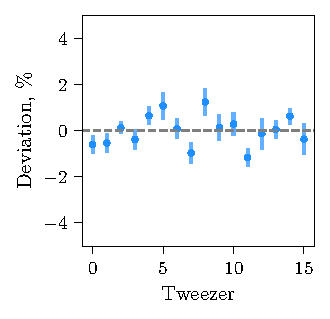
\includegraphics{fig-py/step-plot-balance.pdf} % 0.6 +- 0.2
    % 
    % 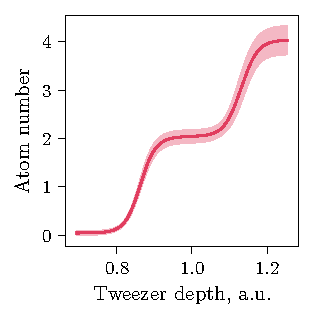
\includegraphics{fig-py/step-plot.pdf}
    % 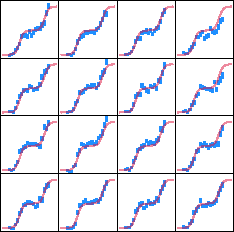
\includegraphics{fig-py/step-plot-inset.pdf}
    \caption{
        \textbf{Step plot.}
        (a) 
        Atom number as a function of tweezer depth during the spilling sequence. 
        % Plateaus correspond to quantized energy levels of the 1D harmonic oscillator. 
        Step plots for each tweezer in the $4 \times 4$ array are shown on the right. The average fit is shown as a solid red line, with standard deviation across sites indicated by the shaded area. 
        (b) Relative deviation of the fitted sigmoid centers for each tweezer after SVF balancing. The standard deviation is $0.7(2)\%$, which is well within the plateau width ($\pm 5\,\%$), ensuring sufficient uniformity for array-wide spilling. \red{$\chi^2$?}
        % All measurements were performed in this work using atom-based measurements and SVF-balanced tweezer depths.
    }
    \label{fig:stepplot}
\end{figure}



\newpage

\begin{figure}[h!]
    \centering
    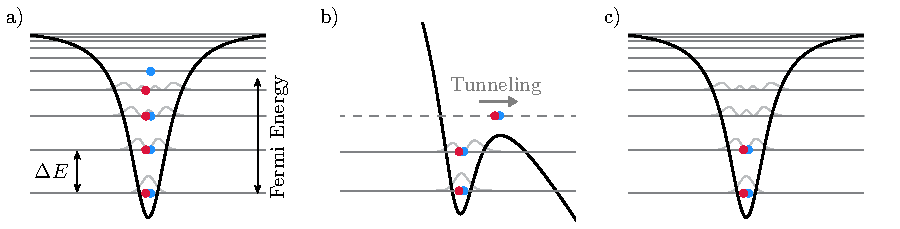
\includegraphics{fig-ai/preparation.pdf}
    \caption{
        \textbf{Deterministic preparation via spilling.}
        (a) Fermionic atoms are initially loaded into a tightly confined optical tweezer, forming a Fermi sea occupying the approximately 1D harmonic oscillator levels up to the Fermi energy. 
        (b) A magnetic field gradient tilts the potential, and the trap depth is lowered such that atoms above a defined spill level tunnel out. 
        (c) This procedure leaves a well-defined number of atoms in the lowest energy states, with a preparation fidelity of approximately 95\%. 
        Blue and red dots denote atoms in different spin states; gray curves indicate the bound-state wavefunctions.
    }
    \label{fig:preparation}
\end{figure}


\begin{figure}[h!]
    \centering
    \addletter{170}{a}
    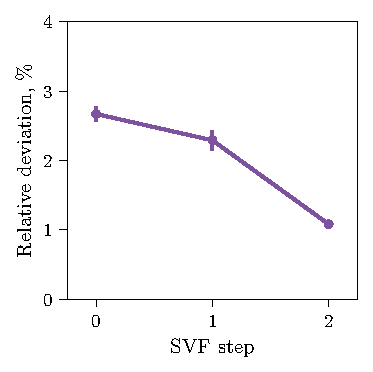
\includegraphics{fig-py/svf-avg.pdf}
    \addletter{170}{b}
    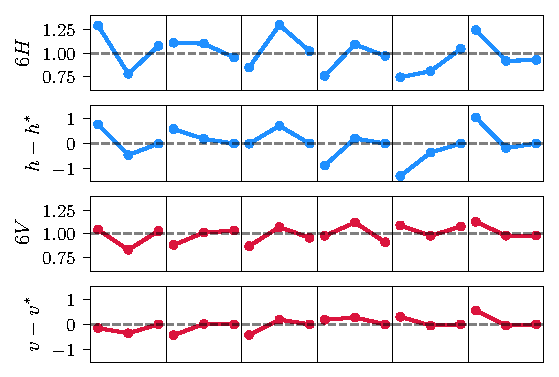
\includegraphics{fig-py/svf.pdf}
    \caption{
        \textbf{Single-value feedback (SVF) optimization for a $6 \times 6$ tweezer array.}
        (a) Relative deviation of effective powers $P_j$ across the array during successive SVF steps, quantified as $\mathrm{std}(P_j)/\langle P_j \rangle$. The initial point corresponds to camera-based balancing; subsequent iterations apply SVF with feedback rates $\gamma = 1/20$ and $\gamma = 1/40$. Further iterations did not yield statistically significant improvements. 
        (b) Retrieved horizontal powers $H_i$ and vertical powers $V_j$ (top and third rows), along with corresponding deviations of driving amplitudes from their final target values, $h - h^*$ and $v - v^*$. The recovered $H$, $V$ vectors are extracted from the photon count matrix $M_{ij}$ using factorization as described in \eqref{uv-decomposition}.
    }
    \label{fig:svf}
\end{figure}


\newpage

\begin{figure}[h!]
    \centering
    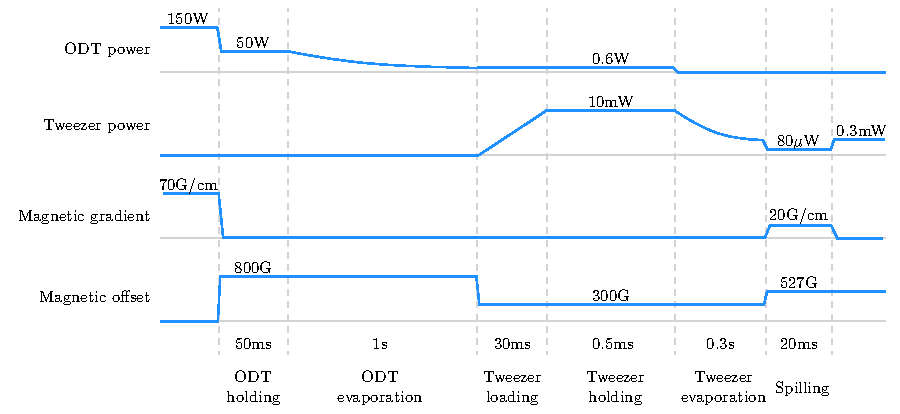
\includegraphics{fig-ai/preparation-seq.pdf}
    \caption{
        \textbf{Experimental sequence for deterministic atom number preparation.} 
        After loading a spin-balanced mixture into a crossed ODT from the MOT, we perform two-stage evaporation in the ODT. The atoms are then transferred into an optical tweezer via an adiabatic ramp. Further evaporation is carried out in the tweezer before executing the spilling procedure. Spilling takes place at 527\,G and a magnetic field gradient of 20\,G/cm to remove atoms above the spill level. The full sequence enables high-fidelity few-body preparation within a sub-2\,s cycle time. A detailed description can be found in~\cite{culemann_construction_2024}.
    }
    \label{fig:preparationseq}
\end{figure}



\begin{figure}[h!]
    \centering
    \addletter{145}{a}
    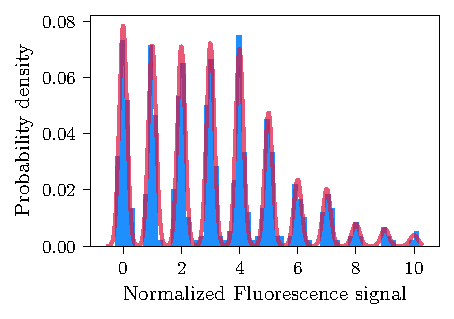
\includegraphics{fig-py/atom-counting.pdf}
    \phantom{4242}
    \addletter{145}{b}
    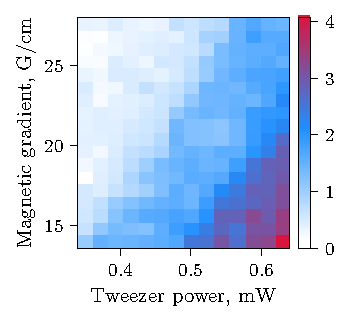
\includegraphics{fig-py/step-plot-2d.pdf}
    \caption{
        (a) Calibration histogram for single-atom counting based on fluorescence signal after after loading to the MOT. Clear quantized peaks correspond to integer atom numbers; the solid red line is a multi-Gaussian fit to the distribution. 
        (b) Measured 2D step plot as a function of tweezer power and magnetic field gradient. Each point indicates the average atom number obtained for a given combination of parameters. This map confirms that for any spill power, a suitable magnetic gradient can be found to achieve a desired quantized atom number.
    }
    \label{fig:spillingadd}
\end{figure}


% \newpage

% \begin{figure}[h]
%     \centering
%     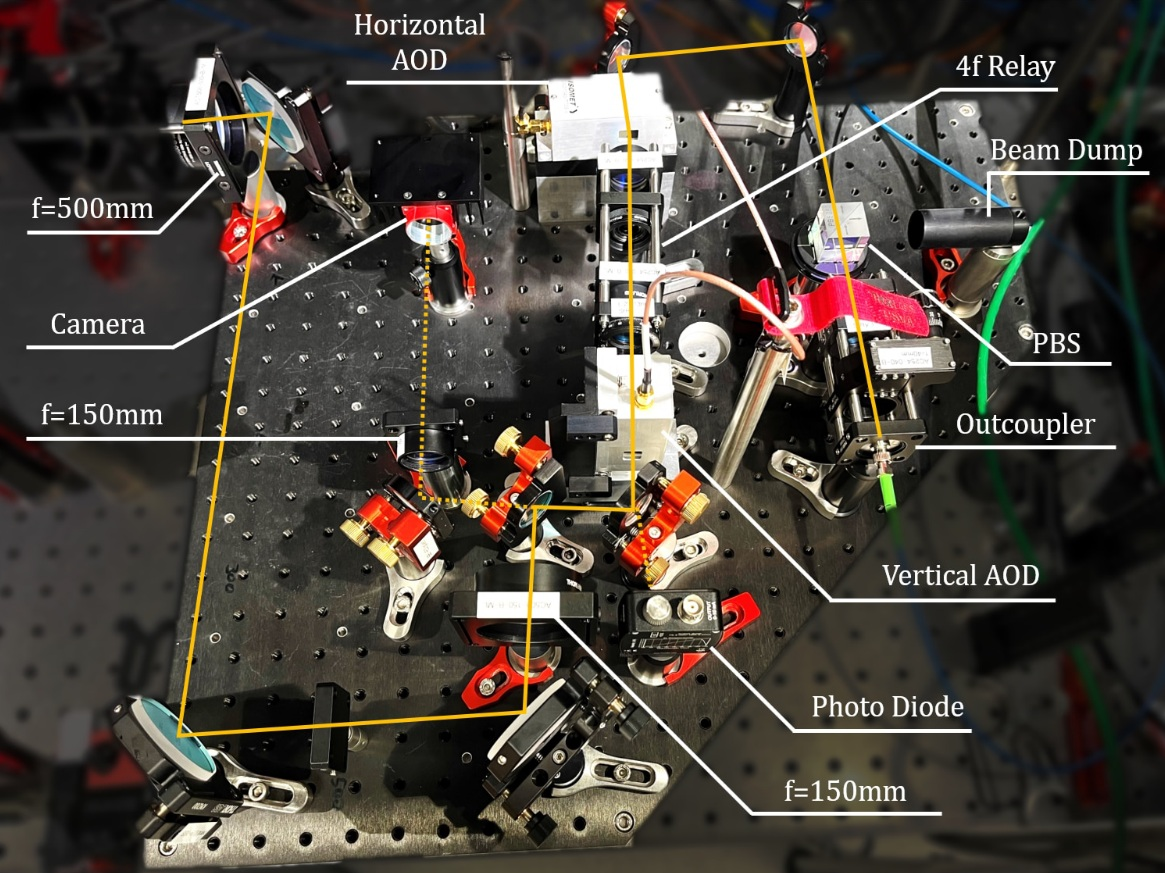
\includegraphics[width=0.5\textwidth]{imgs/tw-setup.jpg}
%     \caption{
%     \textbf{Optical setup for 2D tweezer array.} 
%     The beam path (solid orange line) includes two orthogonal AODs, a $4f$ relay, and diagnostic components. Dashed lines indicate monitoring light paths. Taken from \cite{culemann_construction_2024}.
%     }
%     \label{fig:tw-setup}
% \end{figure}



\newpage


\begin{figure}[h]
    \centering
    \addletter{130}{a}
    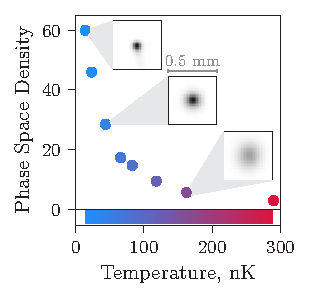
\includegraphics{fig-ai/m-bec-1-joined.pdf}
    \addletter{130}{b}
    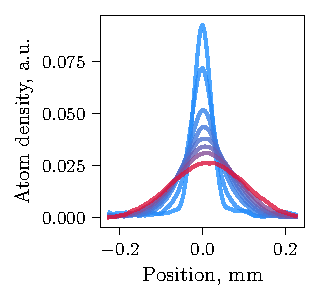
\includegraphics{fig-py/m-bec-2.pdf}
    \addletter{130}{c}
    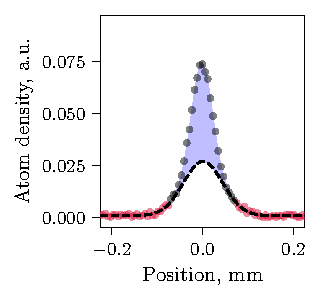
\includegraphics{fig-py/m-bec-3.pdf}
    \caption{
        \textbf{Molecular Bose-Einstein condensate data.}
        (a) Phase space density (PSD) increases as temperature decreases via evaporative cooling, indicating condensation onset. 
        (b) Atom density profiles normalized to unit area; color encodes temperature as in (a).
        (c) At low temperature, the profile shows a bimodal shape: a Gaussian fit to thermal wings (red dots) underestimates the central peak, revealing the mBEC component (blue area).
    }
    \label{fig:mbec}
\end{figure}


\begin{figure}[h]
    \centering
    % 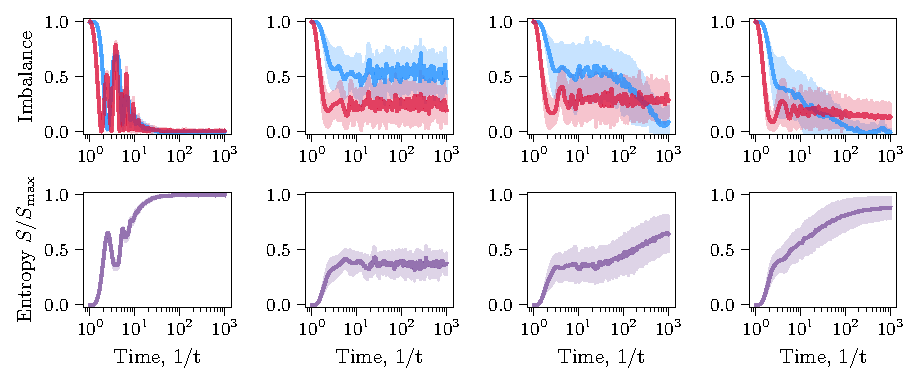
\includegraphics{fig-py/loc-therm.pdf}
    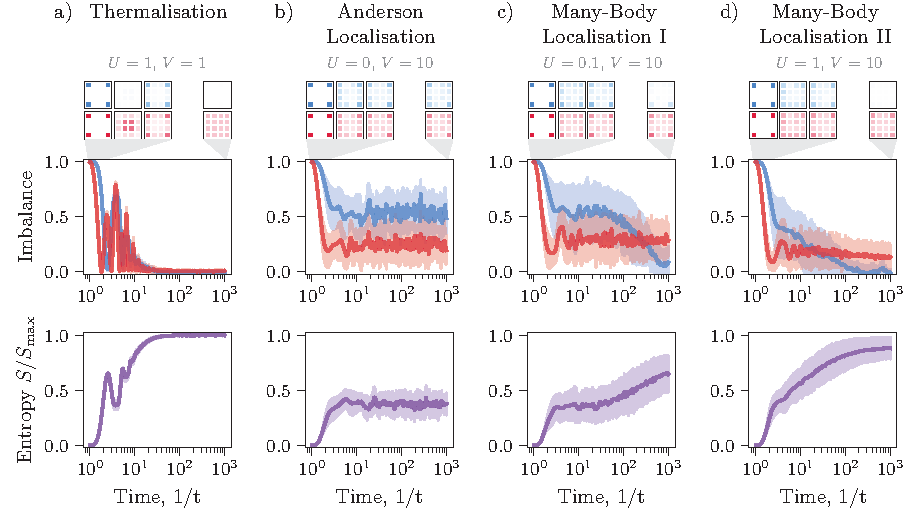
\includegraphics{fig-ai/loc-therm.pdf}
    \caption{
        \textbf{Dynamical phases in a 2D Fermi-Hubbard system.} 
        \textit{Top}: Snapshots of particle density (red) and magnetization magnitude (blue). 
        \textit{Middle}: Time evolution of density imbalance (red) between corners and bulk, and subsystem magnetization (blue). 
        \textit{Bottom}: Normalized entanglement entropy evolution. 
        All results are averaged over 10 noise realizations; shaded areas indicate standard deviation across realizations.
        Data were obtained using ED.
        % Parameters: (a) $U=1, V=1$, (b) $U=0, V=10$, (c) $U=0.1, V=10$, (d) $U=1, V=10$.
        % \\ \textit{Parameters:} (a) $(1,1)$, (b) $(0,10)$, (c) $(0.1,10)$, (d) $(1,10)$ for $(U,V)$.
    }
    \label{fig:loctherm}
\end{figure}

 

\newpage




\begin{figure}[h]
    \centering
    \addletter{195}{a} \phantom{4}
    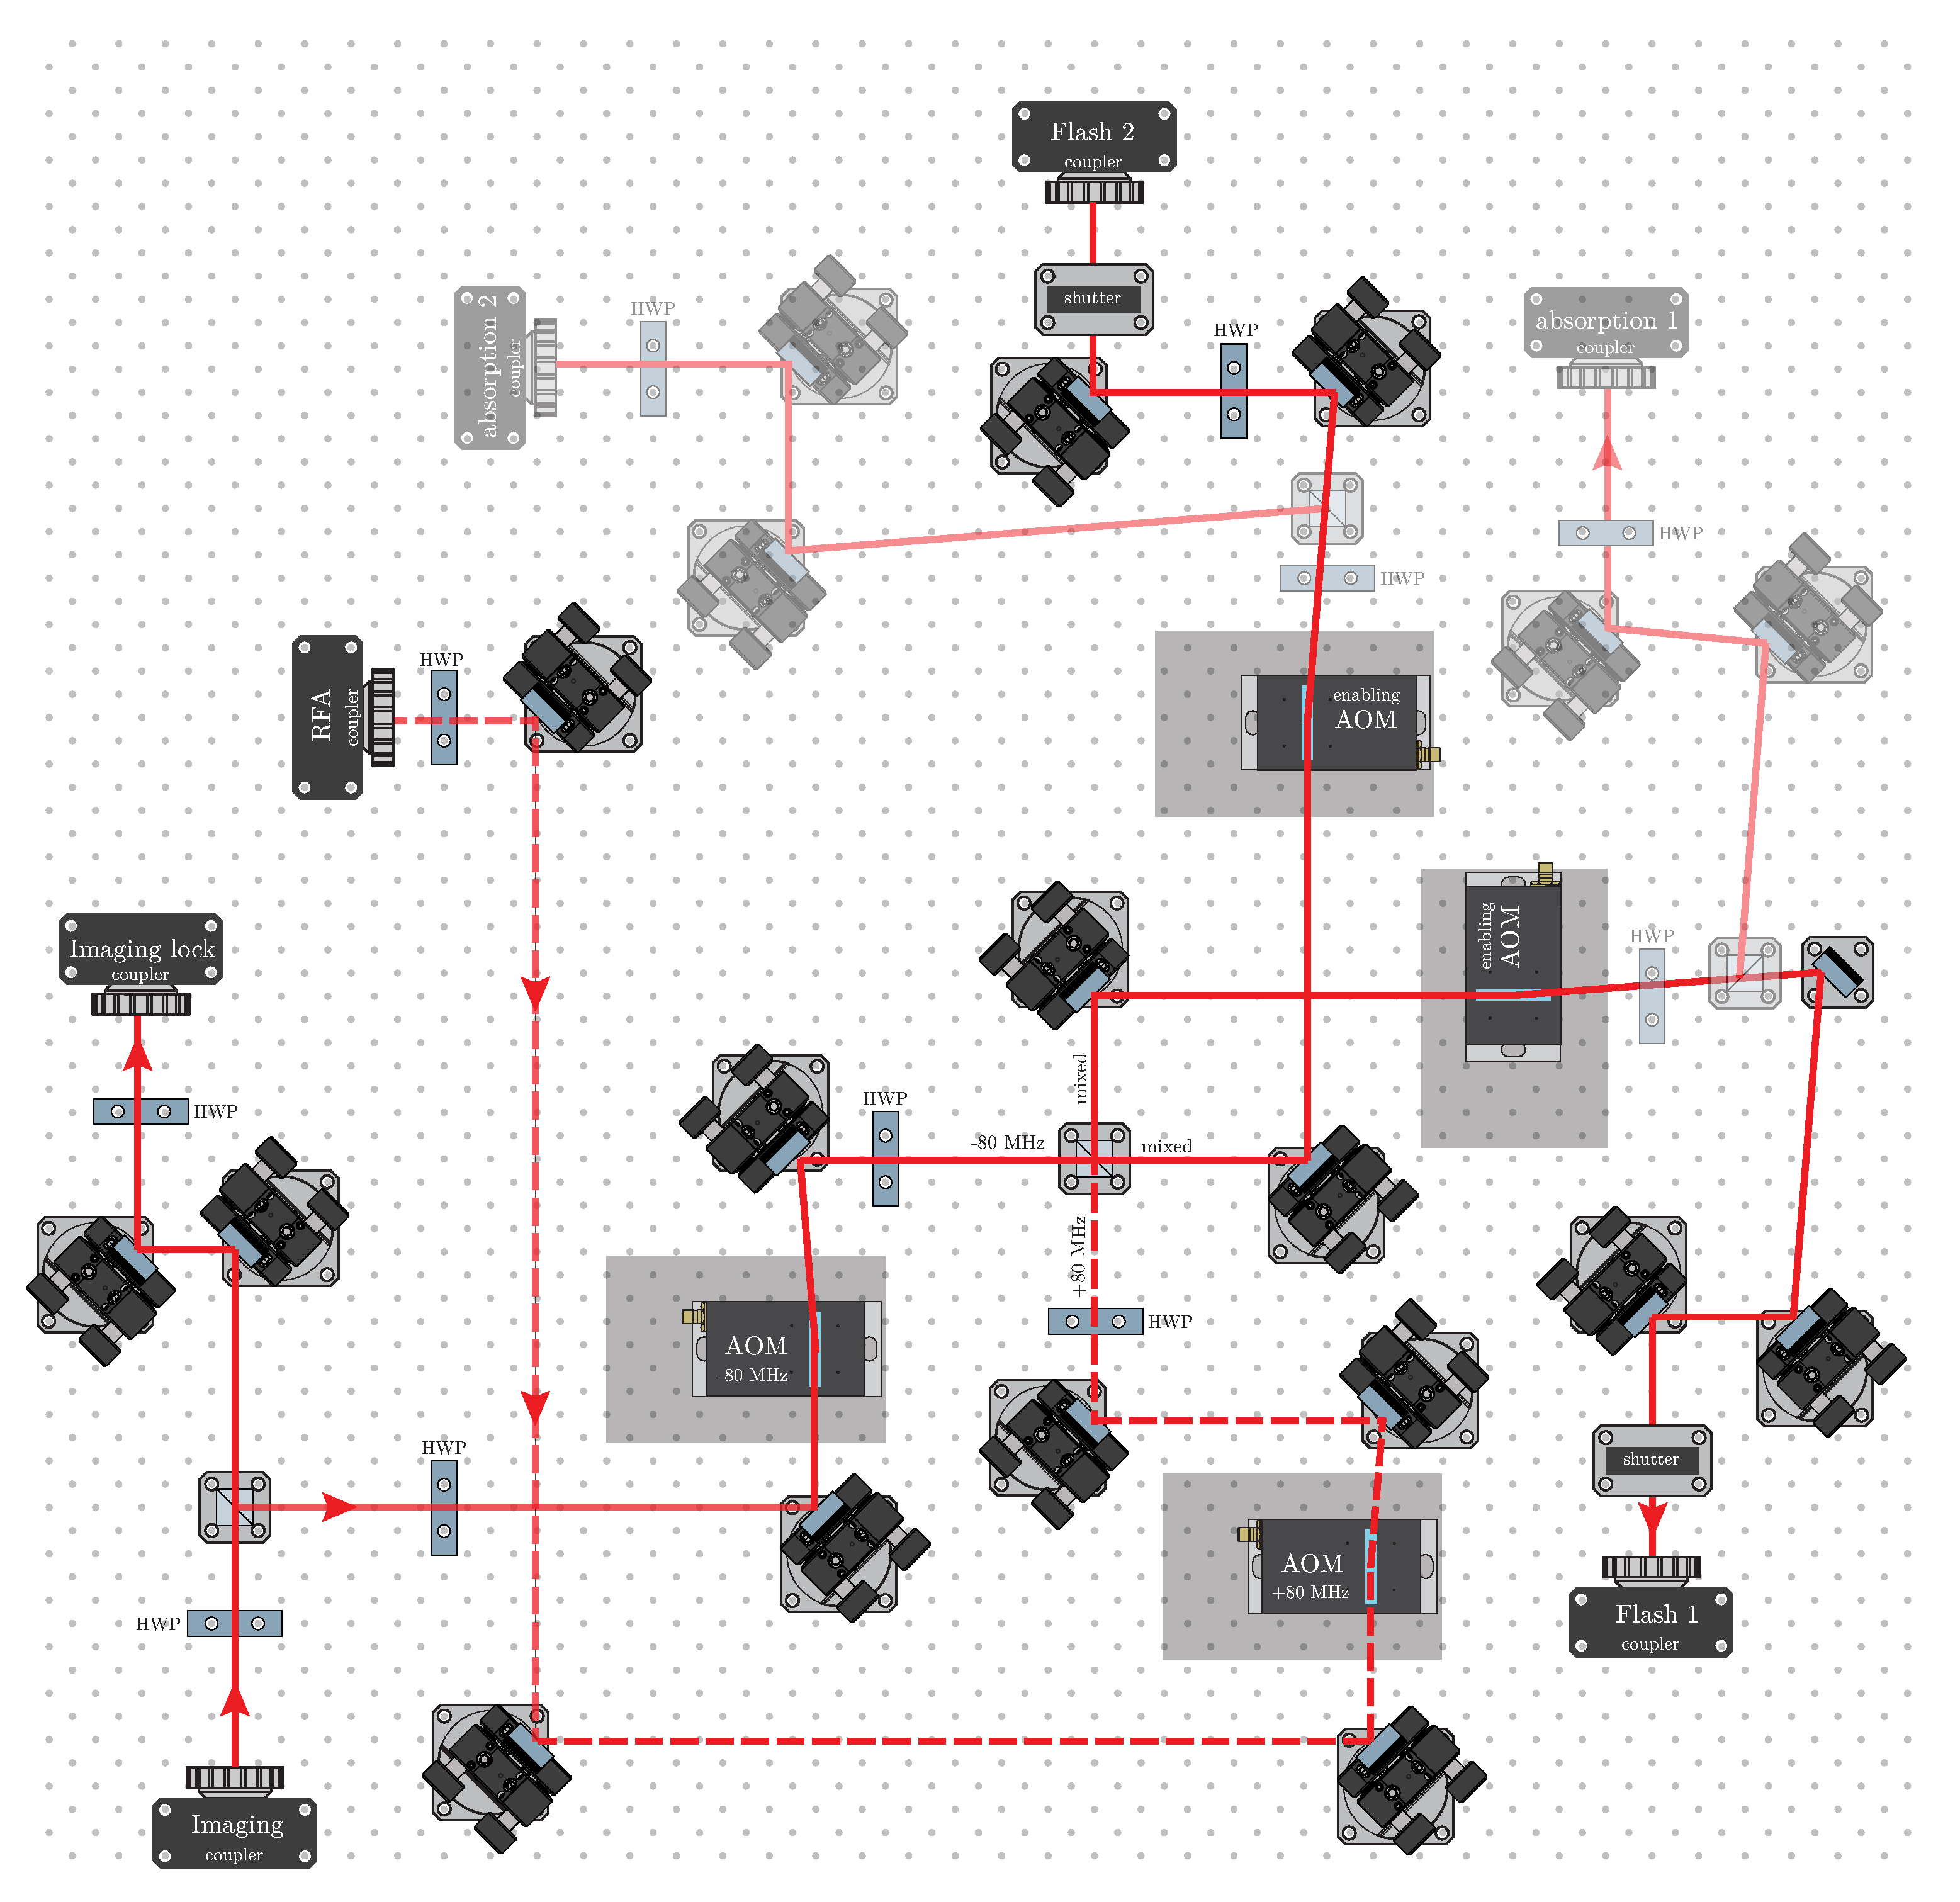
\includegraphics[width=0.4\textwidth]{fig-ai/flashing-distribution-scheme.pdf}
    \hspace{10 mm} 
    \addletter{195}{b} \phantom{4}
    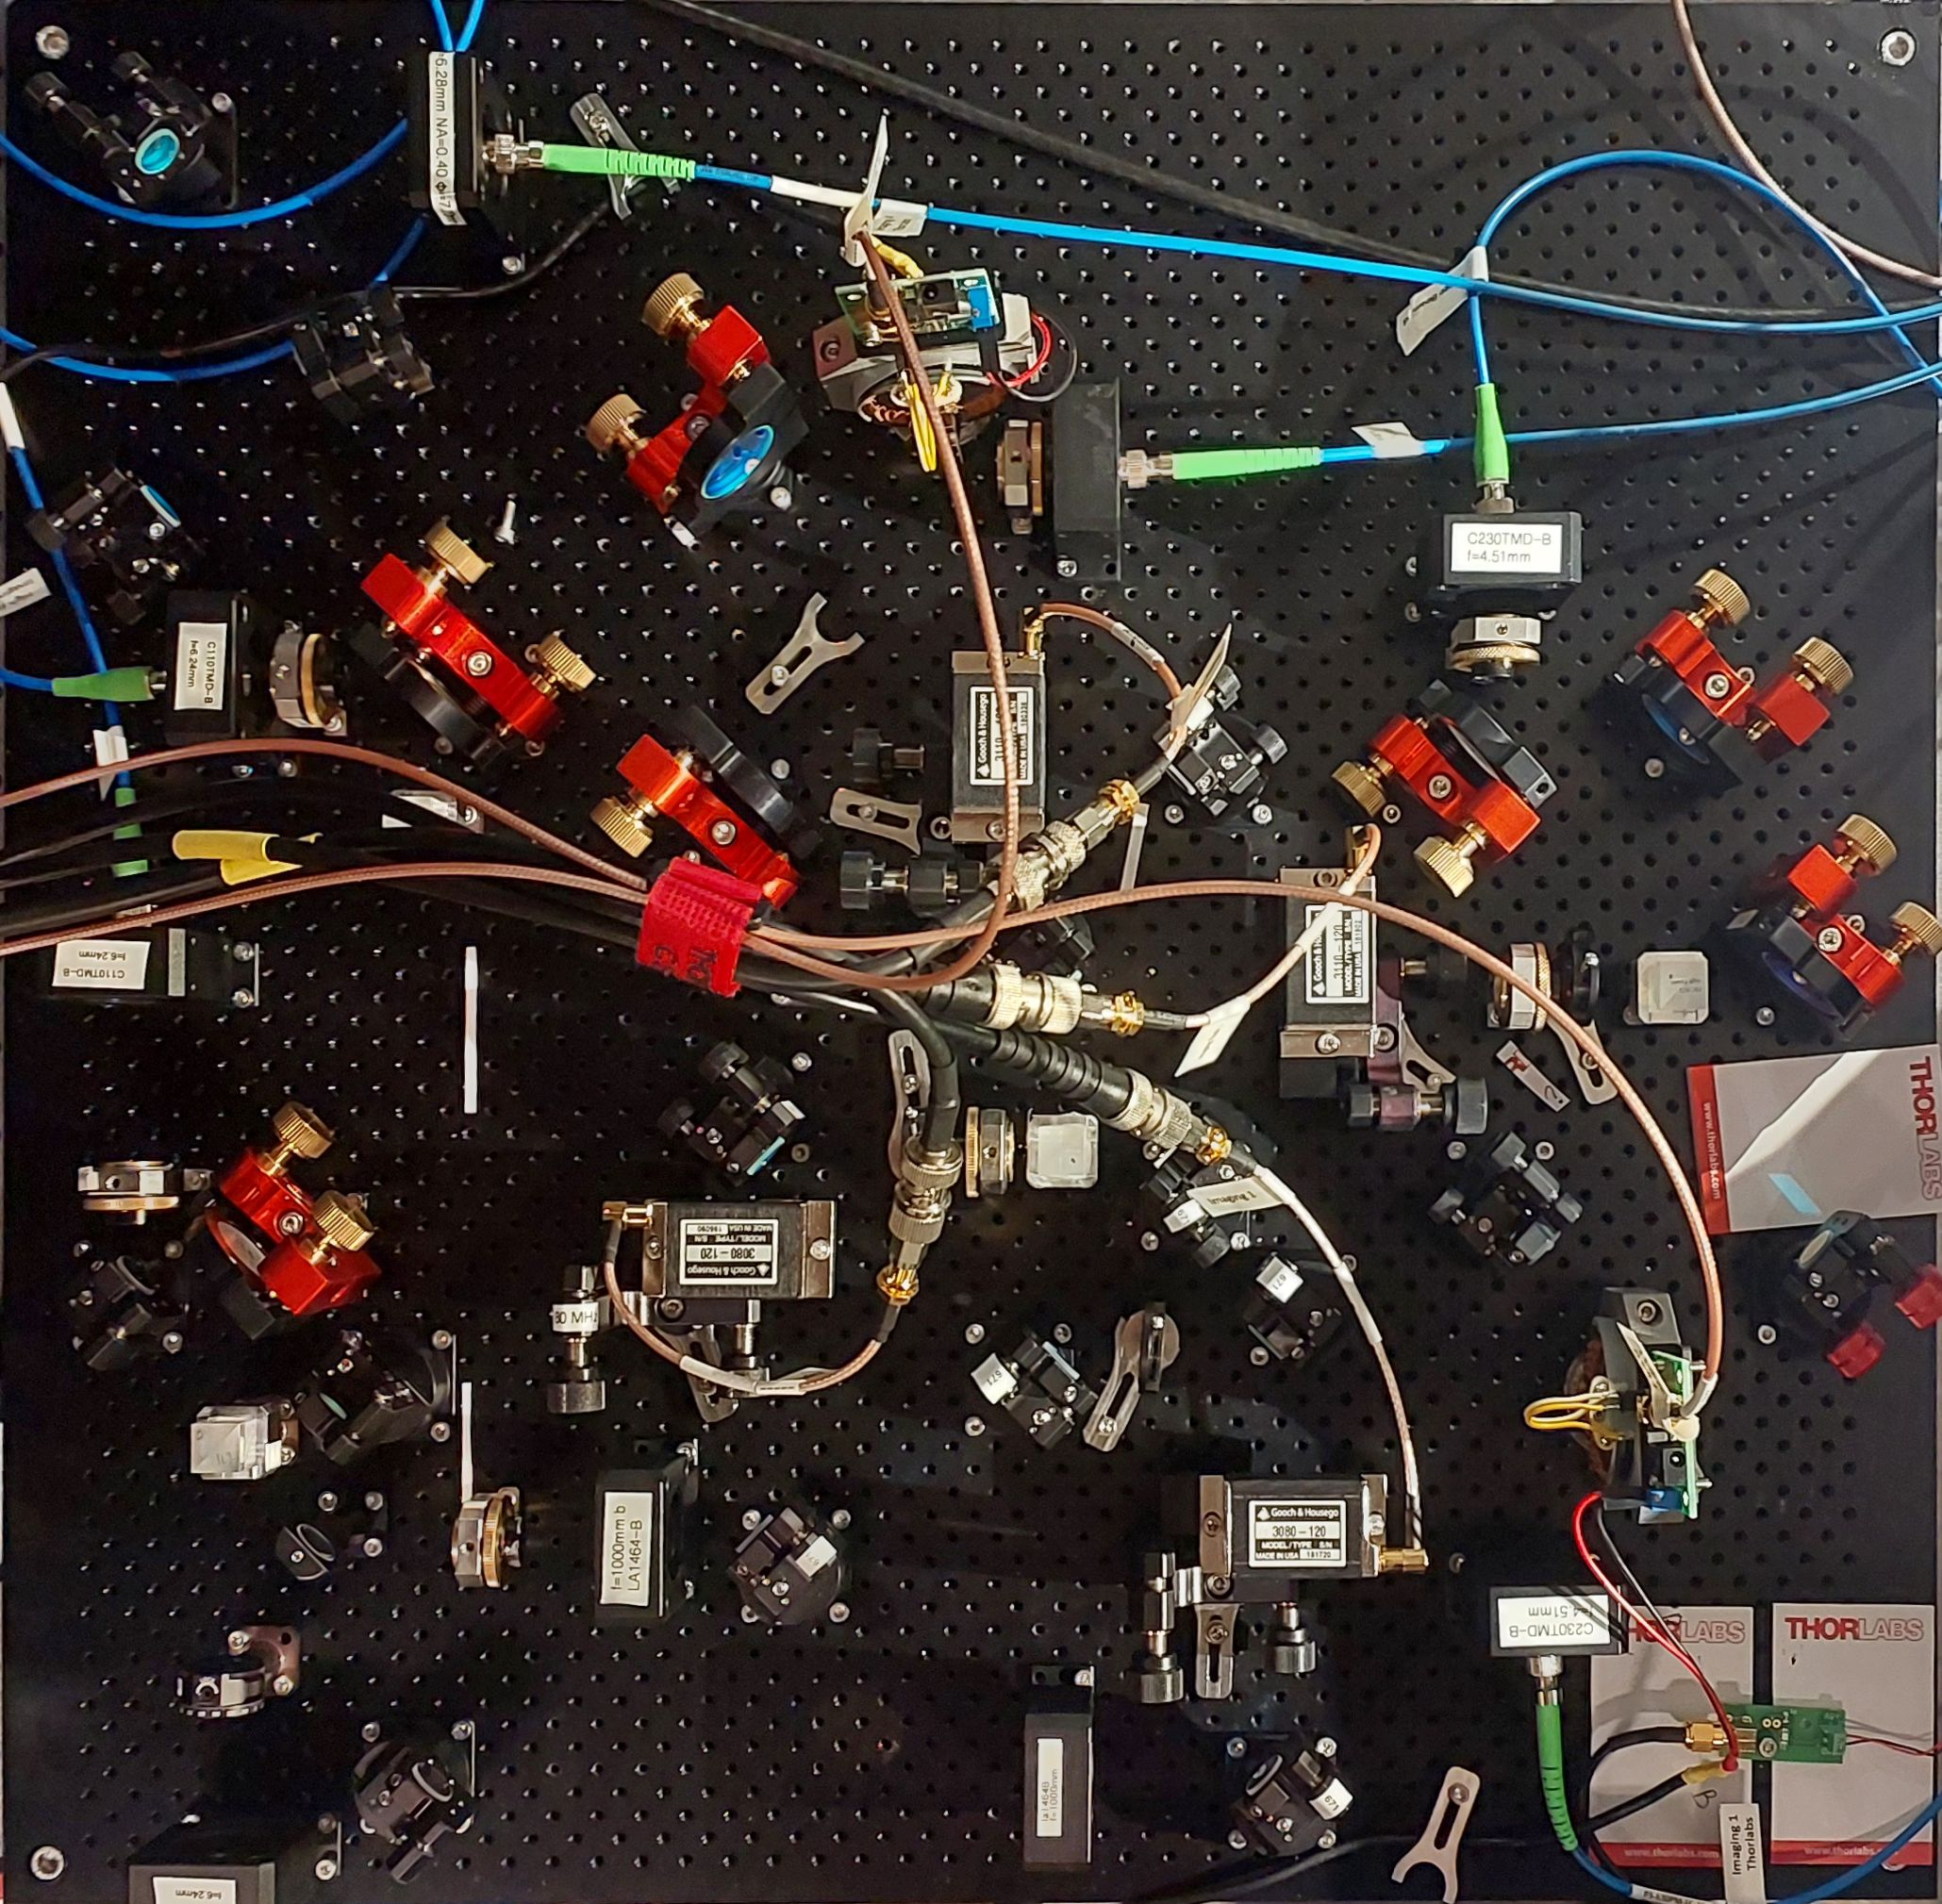
\includegraphics[width=0.4\textwidth]{imgs/flashing-distribution-img.jpg}

    \addletter{90}{c}
    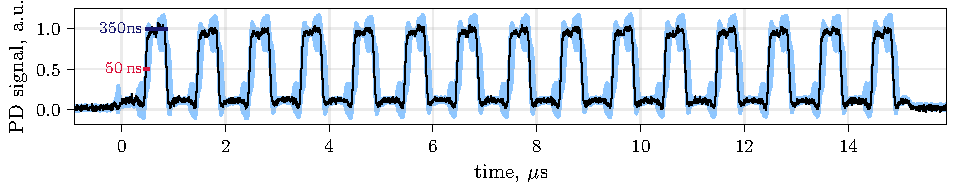
\includegraphics{fig-py/flashing-oscilloscope.pdf}

    \caption{
        \textbf{Distribution board for flashing}. 
        a) Optical layout of the board used to combine and control light for free-space imaging states $\ket{3}$ and $\ket{6}$.
        b) Experimental implementation.
        c) PD signal of the flashing measured on an oscilloscope (black -- a single experimental run, blue -- the standard deviation over 20 runs, red -- rise time).
    }
    \label{fig:flashing}
\end{figure}


\begin{figure}[h]
    \centering
    \addletter{105}{a} \phantom{4}
    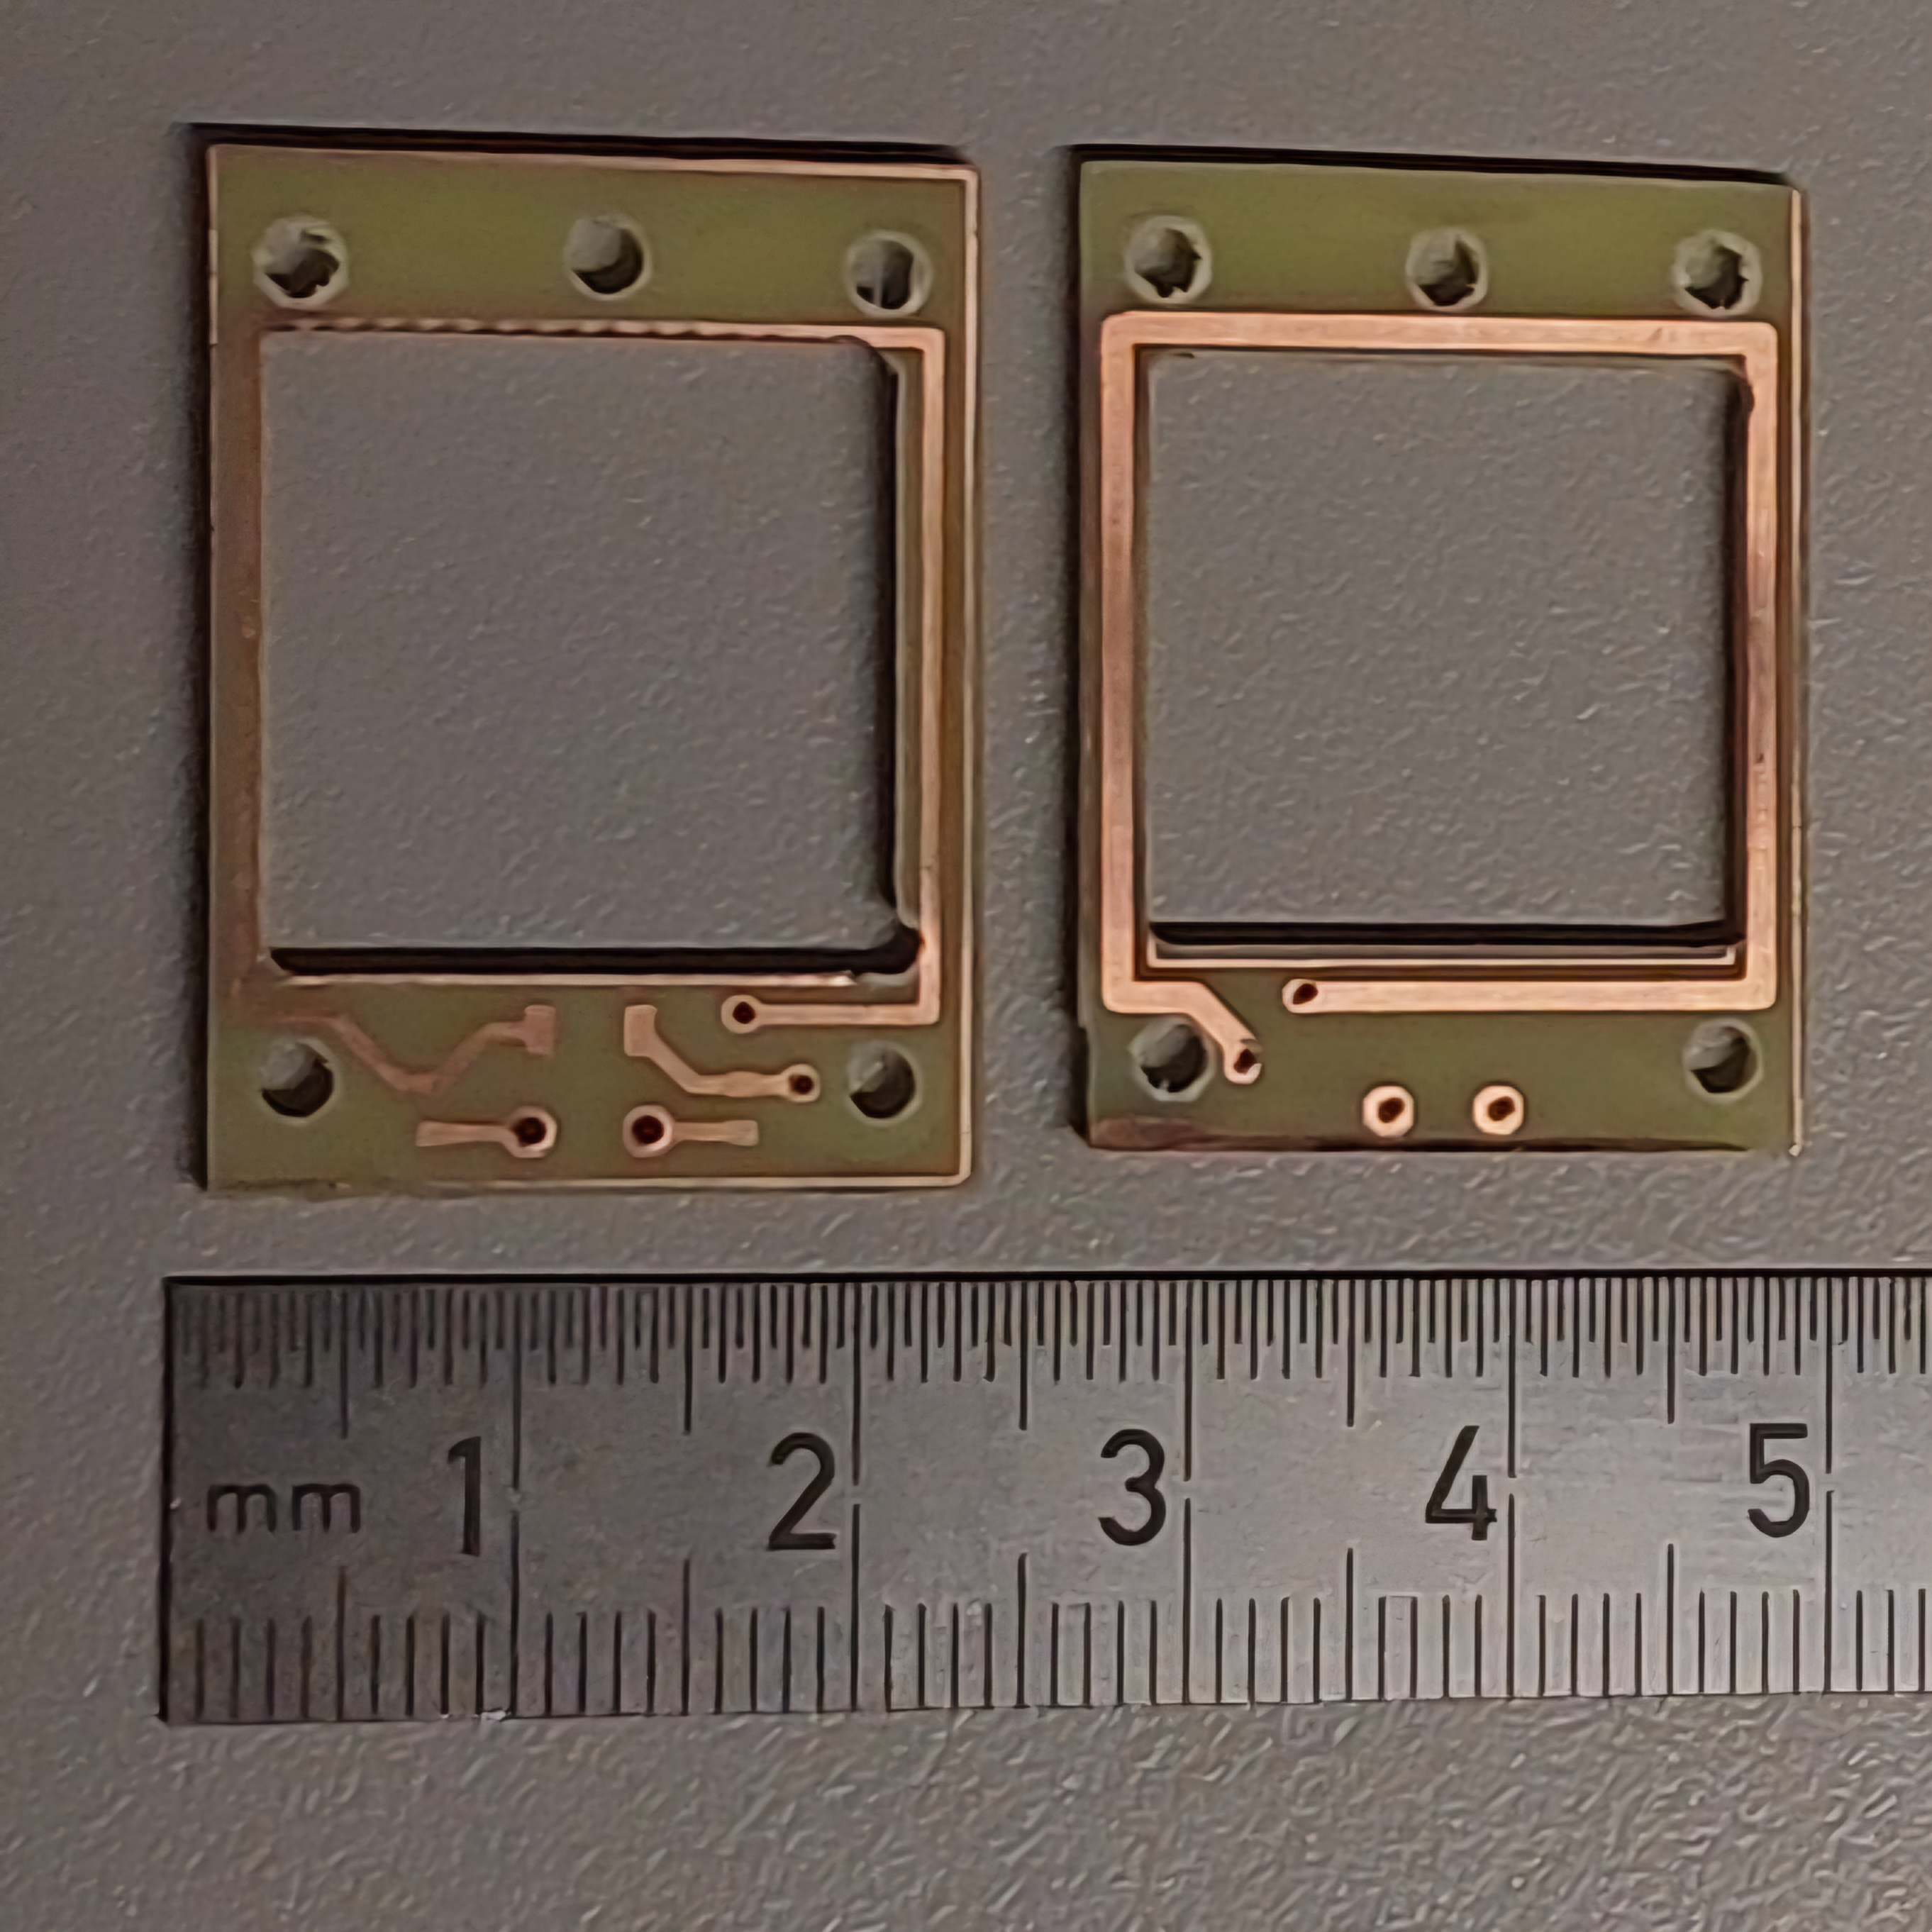
\includegraphics[width=1.5in]{imgs/RF.jpg}
    \hspace{1cm}
    \addletter{105}{b} \phantom{4}
    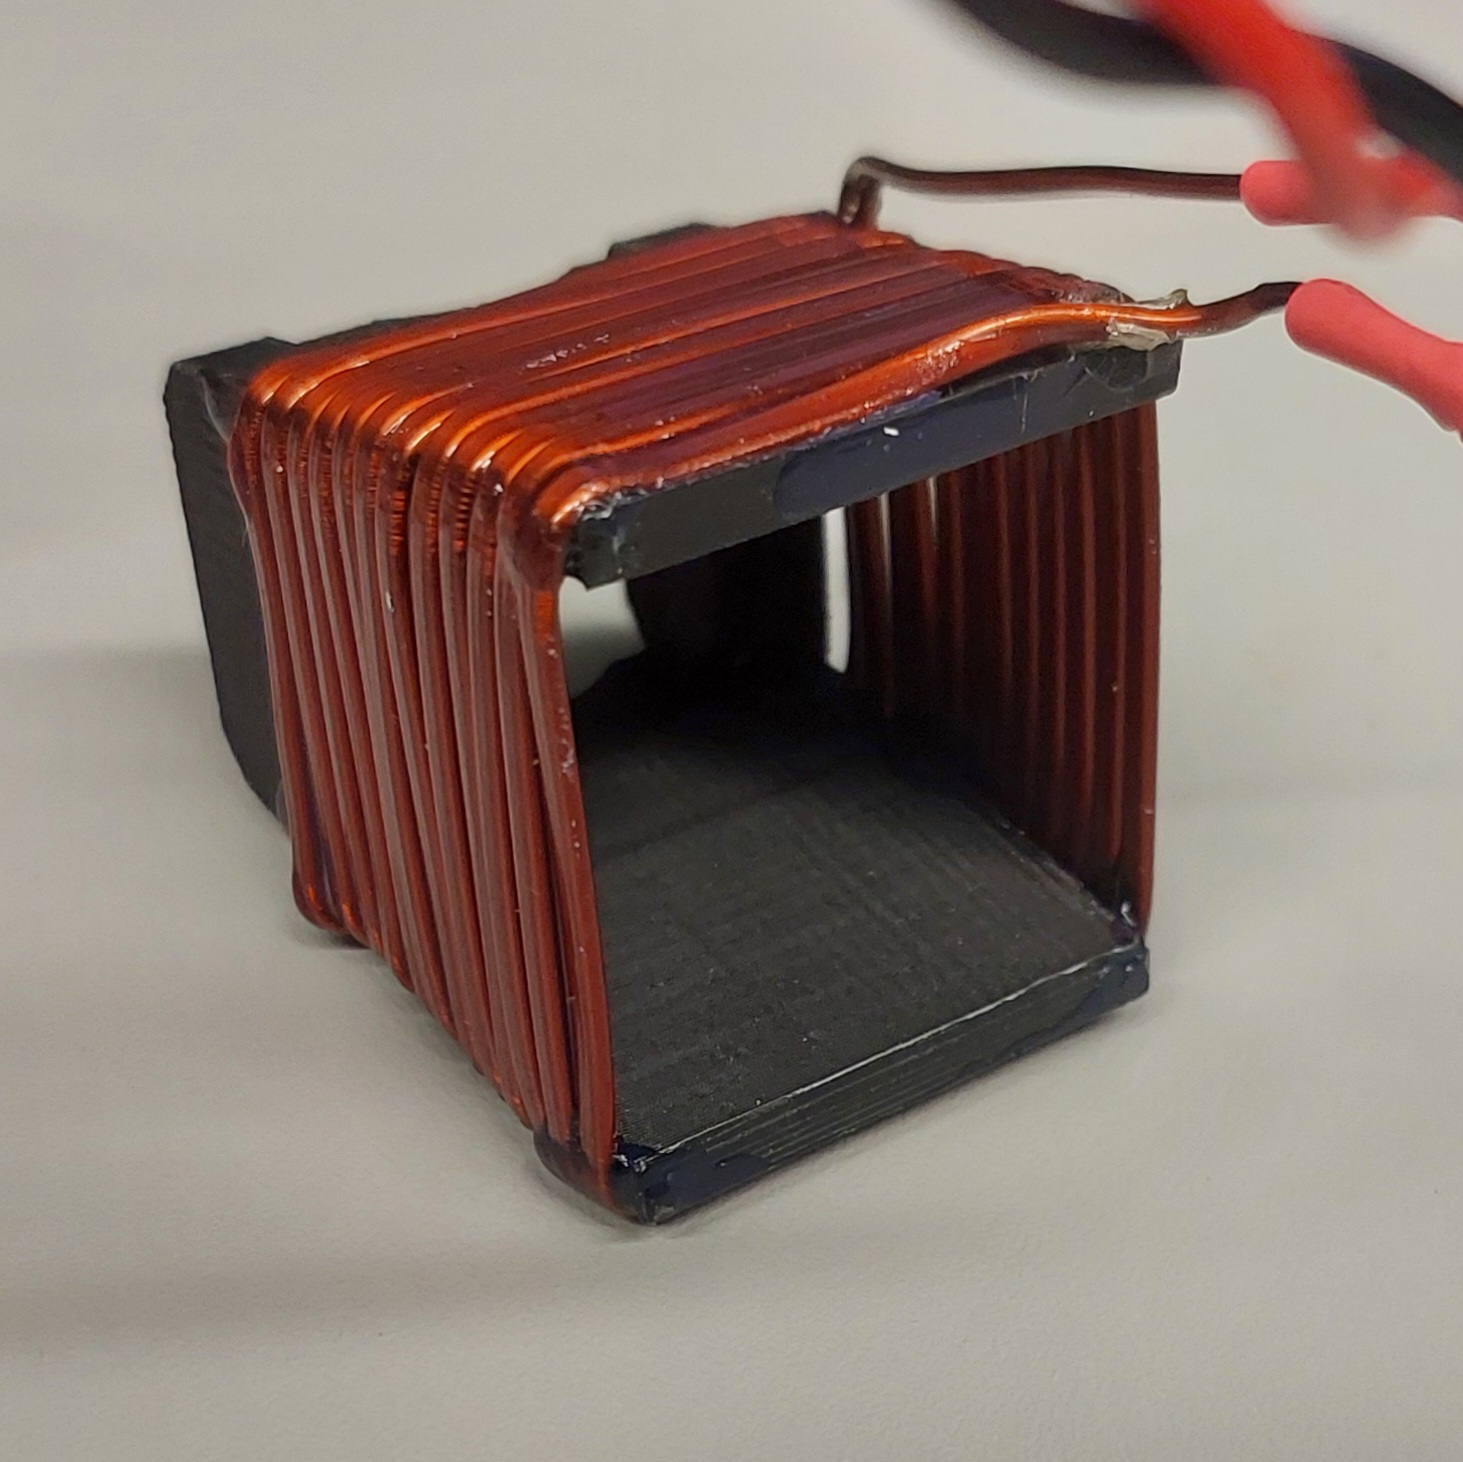
\includegraphics[width=1.5in]{imgs/MW.jpg}
    \caption{
        \textbf{RF and MW antennas used for spin control.}
        (a) PCB-based radiofrequency (RF) antenna used for driving spin transitions at MHz frequencies. 
        (b) Microwave (MW) loop antenna, designed to efficiently couple to hyperfine transitions in $^6$Li. 
        These antennas are used for coherent spin manipulation.
        % performance characterization via spin-flip fidelity is discussed in the following figures.
    }
    \label{fig:rfmw}
\end{figure}








% \begin{figure}
%     \centering
%     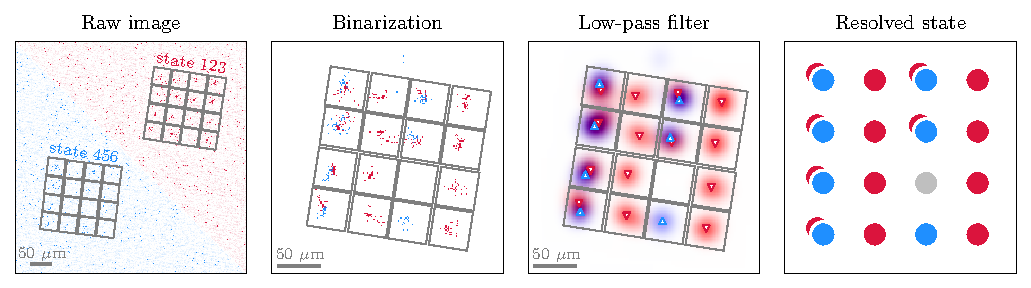
\includegraphics{fig-py/imaging-spin-resolved.pdf}
%     \caption{
%         \textbf{Spin-resolved single-atom imaging.}
%         Spatially separated $\sigma_+$ and $\sigma_-$ fluorescence is imaged onto two distinct regions of the camera. The binarization step identifies photon counts above a threshold, followed by a low-pass filter to extract spatially localized signals. Final spin states are assigned based on relative signal strength in each channel:
%         \raisebox{-1pt}{\scalebox{1.5}{\textcolor{ublue}{\textbullet}}} -- $\ket{1}$, 
%         \raisebox{-1pt}{\scalebox{1.5}{\textcolor{ured}{\textbullet}}} -- $\ket{2}$, 
%         \raisebox{-1pt}{\scalebox{1.5}{\textcolor{uhole}{\textbullet}}} -- no atom.
%     }
%     \label{fig:spin-resolved}
% \end{figure}


% Lorem ipsum dolor sit amet, consectetur adipisicing elit, sed do eiusmod
% tempor incididunt ut labore et dolore magna aliqua. Ut enim ad minim veniam,
% quis nostrud exercitation ullamco laboris nisi ut aliquip ex ea commodo
% consequat. Duis aute irure dolor in reprehenderit in voluptate velit esse
% cillum dolore eu fugiat nulla pariatur. Excepteur sint occaecat cupidatat non
% proident, sunt in culpa qui officia deserunt mollit anim id est laborum.


% \newline
% \phantom{42}
% \newline
% \addletter{100}{c} \phantom{4}
% 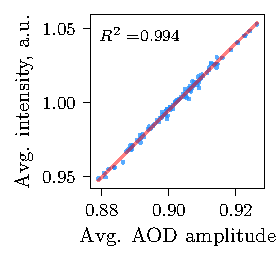
\includegraphics{fig-py/crosstalk-camera-amp.pdf}
% \phantom{4}
% \addletter{100}{d} \phantom{4}
% 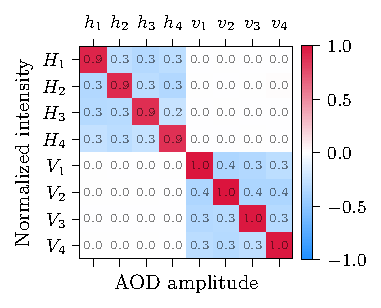
\includegraphics{fig-py/crosstalk-camera.pdf}
% \hfill
% \phantom{4}

